%%%%% CHAPTER SKIN PROPERTIES TO DATA
% \chapter{De propriété physiques de la peau aux données de travail}
\chapter{Des propriétés physiques aux données clinique}
\label{chap:chapter_2}

% SECTION SKIN PROPERTIES
\section{Propriétés de la peau}
Notre perception de la peau est façonnés par divers phénomènes physique d'interaction entre la lumière et ses tissus. Ces derniers influent de par leur structure et de par leur composantes. Nous aborderons cette section de manière descendante, en déroulant le processus d'interaction d'un photon qui entre en contact avec la peau. Ce processus est schématisé de manière macroscopique en \Cref{fig:light_interaction}. La réflexion spéculaire est le premier phénomène pouvant se produire, à l'interface air/peau et est due au changement d'indice de réfraction. Ce faisant, la partie résiduelle parvenue à la peau va interagir avec les diverses structures de la peau et être soit ré émise sans modification de longueur d'onde, nous parlons alors de réflexion diffuse, soit absorbé, nous parlons dans ce cas d'absorption. Cette absorption peut réagir de diverses manière selon la nature du composé et selon la longueur d'onde de l'énergie reçue: 
\begin{inenum}
\item l'énergie peut-être dissipé sous forme de chaleur
\item ou être ré émise avec longueur d'onde différente souvent caractérisé par le terme de fluorescence~\cite{Kollias2002}.
\end{inenum}\par

\begin{figure}[H]
    \centering
    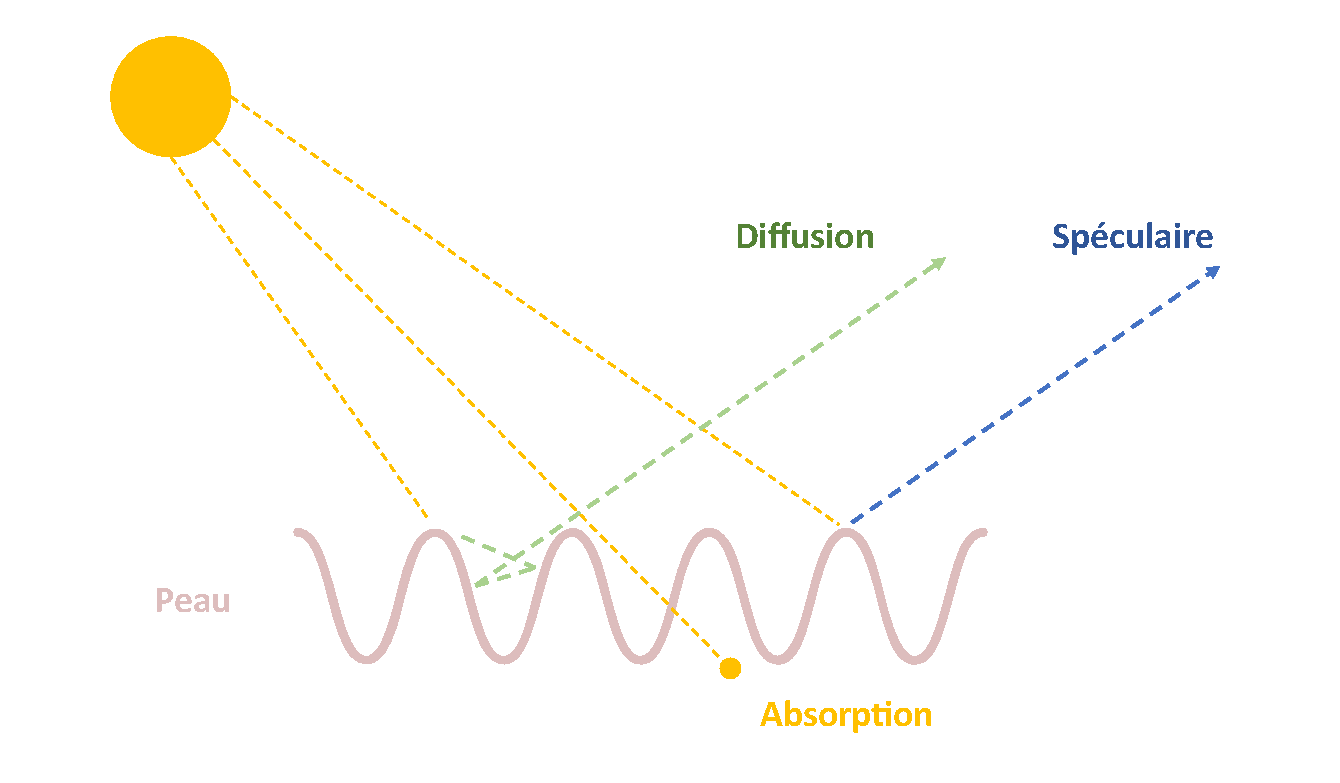
\includegraphics[width=\linewidth]{contents/chapter_2/resources/light_interaction.pdf}
    \caption{Mécanismes d'interaction primaire avec un photon incident.}
    \label{fig:light_interaction}
\end{figure}\par
Dans cette configuration, le choix de la source d'émission de lumière sera l'un des points importants. En effet, comme démontré dans un travail précédent sur les \gls{led} en dermatologie~\cite{Barolet2008}, la longueur d'onde d'émission est un paramètre important quand à la profondeur des structures à observer dans la peau. Ainsi, des longueurs d'onde à l'entrée du spectre visible humain ($\approx$\SI{300}{\nano\metre}) ne parviennent pas à se frayer un chemin en profondeur et ne frôlent que les couches supérieures de l'épiderme, tandis que des longueur d'ondes plus élevée de ce même spectre ($\approx$\SI{900}{\nano\metre}) tendent à atteindre l'hypoderme et ses vaisseaux sanguins. Une synthèse de la pénétration de la lumière en fonction de la longueur d'onde est visible en \Cref{fig:light_penatrating}.\par
\begin{figure}[H]
    \centering
    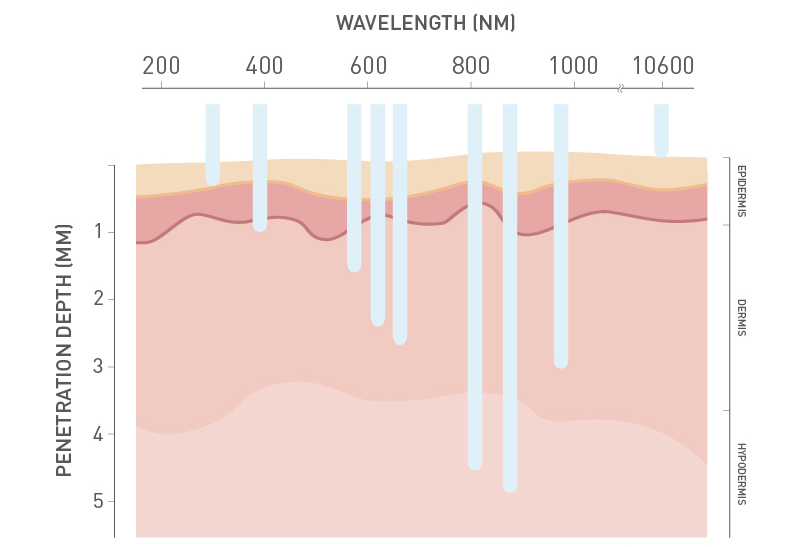
\includegraphics[width=0.8\linewidth]{contents/chapter_2/resources/light_penatrating.png}
    \caption{Schéma représentatif des longueurs d’onde et de leur capacité de pénétration de la peau \cite{Barolet2008}.}
    \label{fig:light_penatrating}
\end{figure}
Outre la question de la profondeur, le choix de la longueur d'onde permet d'interagir avec différents types de chromophores pouvant renseigner l'observateur sur des propriétés locales à la peau. Certains travaux focalisés sur les systèmes lasers et  d'émission en général~\cite{Stewart2013} ont permis de mettre en avant le rapport entre la longueur d'onde et des composés majeurs de la peau tels que l'eau, la mélanine ou l'hémoglobine (oxygénée ou non). Pour illustrer ce propos, la \Cref{fig:light_absorption} synthétise ce rapport entre la longueur d'onde d'émission et l'absorption associée à ces quatre composés. La quantification de ces composés permet de revenir à des fonctions de métabolime\cite{Im2016}
En dehors de cette seule quantification de composées, ces travaux permettent de comprendre des changement de métabolismes liés à des types de pathologies, pouvant par exemple amener à une hypervascularisation.\par
\begin{figure}[H]
    \centering
    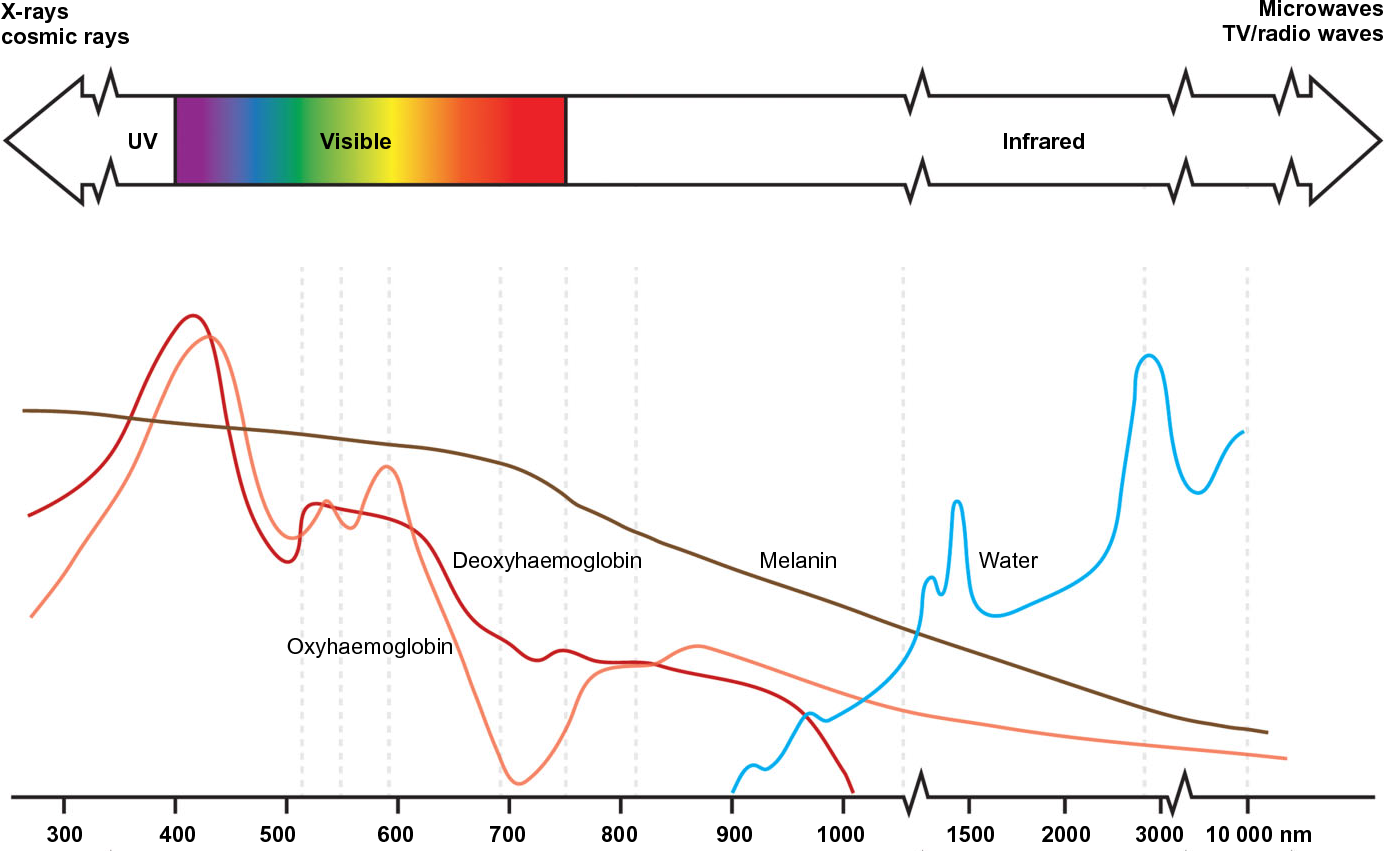
\includegraphics[width=\linewidth]{contents/chapter_2/resources/light_absorption.png}
    \caption{Représentation des longueurs d'ondes et coefficients d'absorption associé selon le type de composé \cite{Stewart2013}.}
    \label{fig:light_absorption}
\end{figure}
 
\clearpage
\section{Modalités d’imagerie non invasives}
Afin de mieux suivre, voire de conserver une trace de leurs patients, les dermatologues disposent de nombreux outils divers. Ils peuvent entre autres dans leur pratique clinique se référer à divers types d’examen que nous distinguerons au travers de deux catégories :
\begin{itemize}
\item D’une part les examens invasifs, pouvant altérer l’organisme du patient à plus ou moins grande échelle. La biopsie est à ce jour le « gold standard » de ce domaine et se réalise par prélèvement et analyse des tissus du patient. Ces techniques sont généralement plus coûteuses à réaliser par unité, nécessitent davantage de temps et peuvent engendrer une gêne voire un risque lors de leur exécution.
\item D’autres part, les examens dit non invasifs, c’est-à-dire ne provoquant pas d’effraction des tissus de la peau parmi lesquels les « imageurs », dispositifs capables de nous restituer une image de différente nature selon le phénomène physique observé. Les coûts peuvent être plus ou moins élevées selon le type de dispositif utilisé et ne procurent en général pas d’inconfort particulier pour la plupart.
\end{itemize}\par
Après avoir abordé de manière non exhaustive les majeures pathologies de la peau et quelques principes d'interaction avec la peau, il convient désormais d'aborder les diverses méthodes permettant une observation non invasives. Ces modalités d'imagerie franchissent en majorité le cap du numérique permettant un suivi plus aisé, voire un échange plus rapide entre professionnels, et l’utilisation de traitements automatiques. Nous séparerons ces techniques en deux catégories distinctes: d’une part les techniques de mesure optique et d'autres part les autres dispositifs basées sur une mesures physique indépendante de l'optique.\par

\subsection{Modalités de mesure optique}
\begin{table}[H]
\begin{tabular}{lllll}
\textbf{Technologie}                                                                & \textbf{Mode d’émission} & \textbf{Résolution Spatiale} & \textbf{Profondeur}                   \\ \hline
Imagerie clinique                                                                   & Réflectance              & Lentille dépendant           & Surface                               \\
Dermatoscope                                                                        & Réflectance              & Lentille dépendant           & Surface                               \\
Microscope confocale par réflectance                                                & Réflectance              & \si{\micro\metre}            & \textless{} \SI{200}{\micro\metre}    \\
Tomographie en cohérence optique                                                    & Réflectance              & \si{\micro\metre}            & \SIrange{1}{2}{\milli\metre}          \\
Imagerie spectrale                                                                  & Réflectance              & Lentille dépendant           & \SIrange{0.1}{1}{\milli\metre}        \\
Spectroscopie à réflexion/fluorescence                                              & Réflectance/Fluorescence & Diamètre de la fibre         & \SIrange{0.1}{1}{\milli\metre}        \\
Microscope confocal Raman                                                           & Raman                    & \si{\micro\metre}            & \SI{150}{\milli\metre}                \\
% Réflectance totale atténuée                                                         & ATR                      & Dimension du Crystal         & \textless{} \SI{2}{\micro\metre}      \\
\end{tabular}
\caption{Aperçu des principales modalités de mesure optique utilisés en dermatologie à but clinique ou exéprimentales \cite{Kollias2002}.}
\label{tab:light_absorption}
\end{table}
\subsubsection{Imagerie clinique}
L’examen de dépistage classique est associé en dermatologie à une inspection à l’œil nu exercée par une personne compétente ou sensibilisée à la détection de pathologies. Cette première modalité fait appel à un dispositif de photographie non propre à la dermatologie. Par ailleurs, n’étant pas spécifique à ce domaine, elle constitue la modalité la moins onéreuse de la discipline dans le cadre de l’imagerie des lésions.\par
Cette modalité, avant l’avènement de l’informatique, se basait sur des supports de type argentique. L’évolution de ce matériel vers le numérique, et l’arrivée de systèmes de type \gls{pacs} ont conjointement motivé une transition vers des données dématérialisées.\par
Ce type d’imagerie donne à l’observateur un point de vue subjectif, similaire à une observation à l’œil nu, utile dans le cadre d’un diagnostic à distance ou dans le suivi à long terme d’un patient. Néanmoins, l'un des points faible est le manque de standard concernant le format d'image et de protocole concernant l'acquisition des images: pas de contraintes d'éclairage, ni de contraintes sur le point de vue à adopter au moment de la prise d'image. Ces éléments amènent à une grande diversité de données, comme nous pouvons le voir en \Cref{fig:photography_example}.\par
\begin{figure}[H]
\centering
    \begin{subfigure}{.5\textwidth}
      \centering
      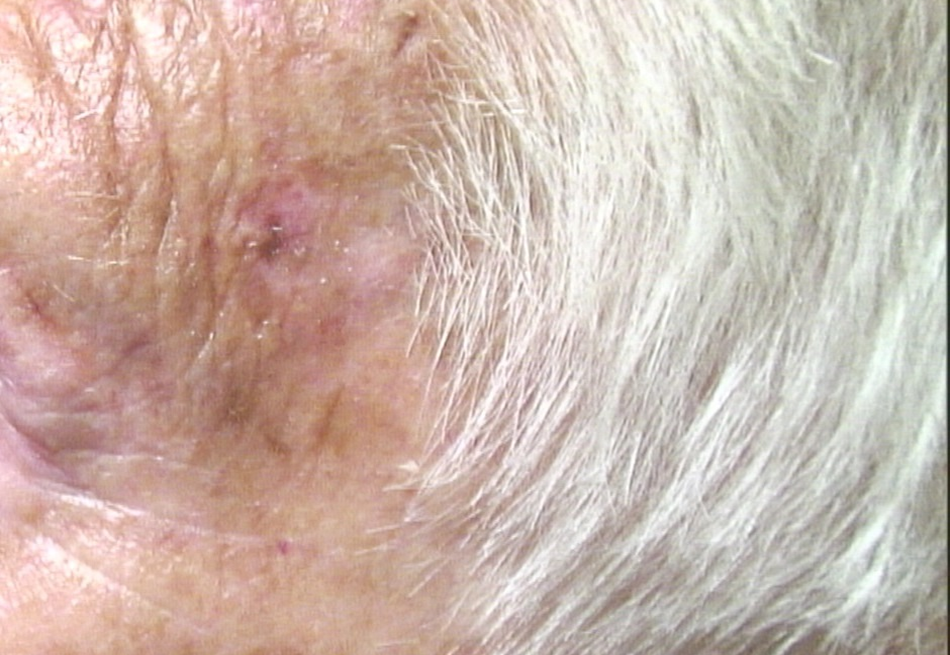
\includegraphics[width=\linewidth]{contents/chapter_2/resources/photography_example_1.png}
    \end{subfigure}
    \begin{subfigure}{.5\textwidth}
      \centering
      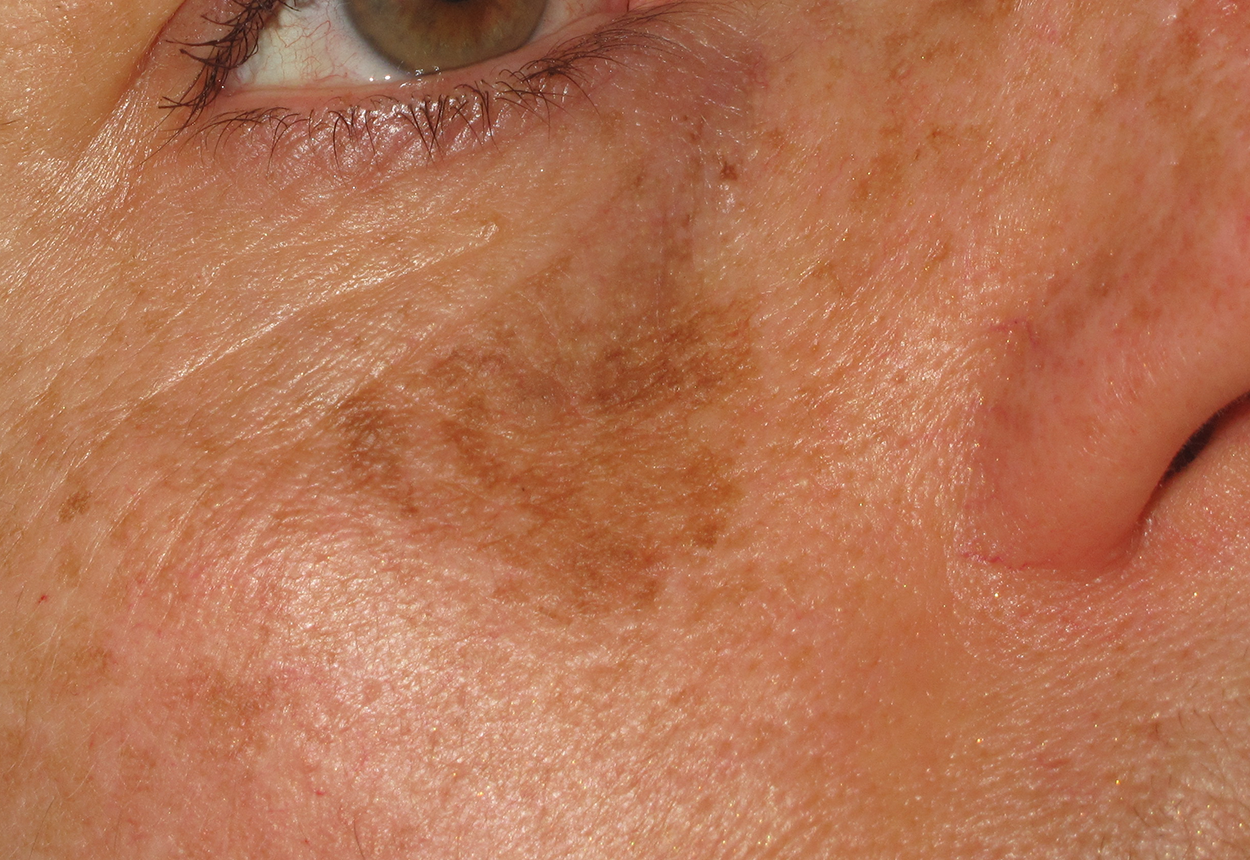
\includegraphics[width=\linewidth]{contents/chapter_2/resources/photography_example_2.png}
    \end{subfigure}
    \caption{Exemple d'images dites de photographie clinique.}
    \label{fig:photography_example}
\end{figure}
\subsubsection{Dermatoscopie}
La dermatoscopie est l'une modalité d’imagerie mise à disposition des praticiens en dermatologie qui a connu son essor durant les années 1980. Également appelé dermatoscopie, microscopie en épiluminescence ou encore microscopie de surface, ce dispositif permet d’observer les lésions cutanées. Cette technique d’imagerie est partiellement attribuée à Johan Christophorus Kohlhaus dont les travaux menés, au XVIIème siècle, sur la microscopie de surface, auraient grandement contribué à initier cette modalité.\par
Cet outil possède comme première caractéristique, de réduire les réflexions de lumière et contribue à rendre le stratum corneum translucide \cite{Katz2001}, permettant ainsi au praticien de visualiser les couches sous-jacentes : épiderme, jonction derme/épiderme ou encore le derme papillaire non visible à l’œil nu. Cette réflexion de lumière était initialement supprimée par l’utilisation d’un fluide (eau, gel, …) entre la peau et le dispositif, mais ce procédé est devenu obsolète sur les derniers modèles avec l’utilisation de lumière  polarisée \cite{Campos-do-Carmo2008}.\par
Une seconde caractéristique non négligeable, est la mise à disposition d’un zoom pouvant varier de 10x à 70x selon la complexité des modèles proposés \cite{Campos-do-Carmo2008}. Cette dernière caractéristique octroie au praticien la possibilité d’appréhender au mieux la structure dans ses moindres détails.\par
De plus, son faible coût d’achat, sa rapidité de diagnostic et son efficacité en comparaison avec le seul œil humain \cite{Lallas2013} contribuent largement  à sa démocratisation dans la profession. Bien qu’utilisé majoritairement dans le dépistage de lésions pigmentaires, son efficacité semble avérée dans le cas de lésions dites non pigmentaires (\gls{bcc} et \gls{scc}) \cite{Lallas2013}. Ces dispositifs tendent à s'adapter de plus en plus à leur marché, s'orientant vers une utilisation tel en \Cref{fig:dermatoscope_example}.\par
\begin{figure}[H]
\centering
    \begin{subfigure}{.33\textwidth}
      \centering
      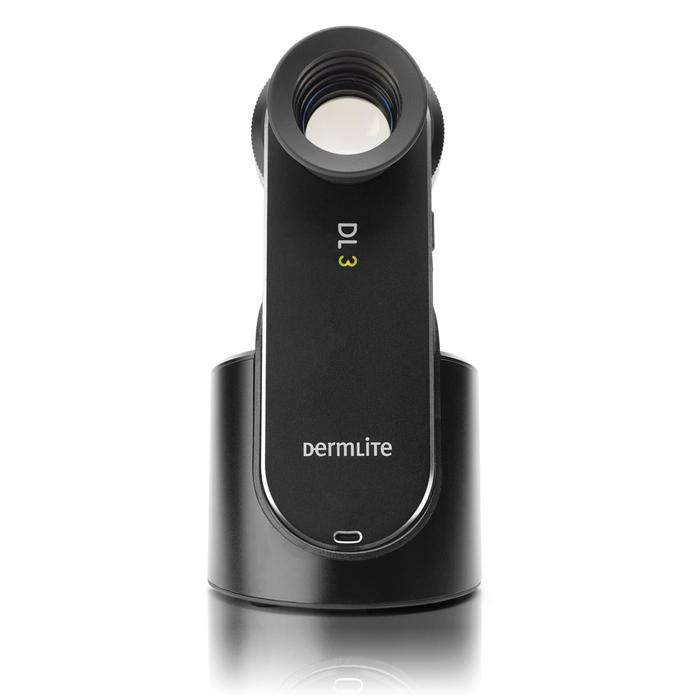
\includegraphics[width=\linewidth]{contents/chapter_2/resources/dermatoscope_example_1.png}
    \end{subfigure}
    \begin{subfigure}{.33\textwidth}
      \centering
      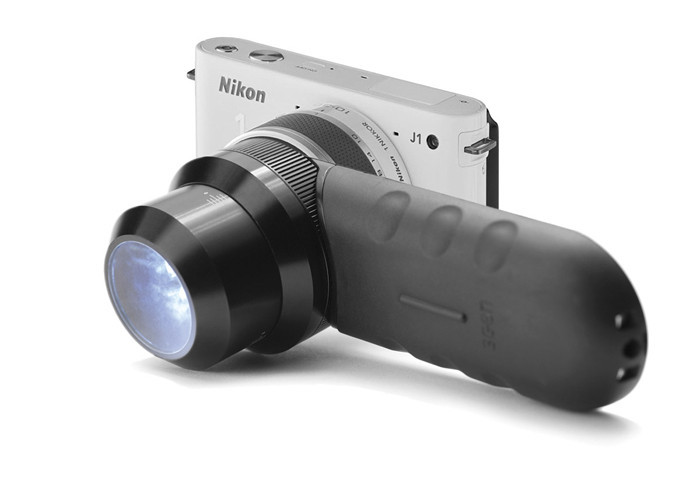
\includegraphics[width=\linewidth]{contents/chapter_2/resources/dermatoscope_example_2.png}
    \end{subfigure}
    \begin{subfigure}{.33\textwidth}
      \centering
      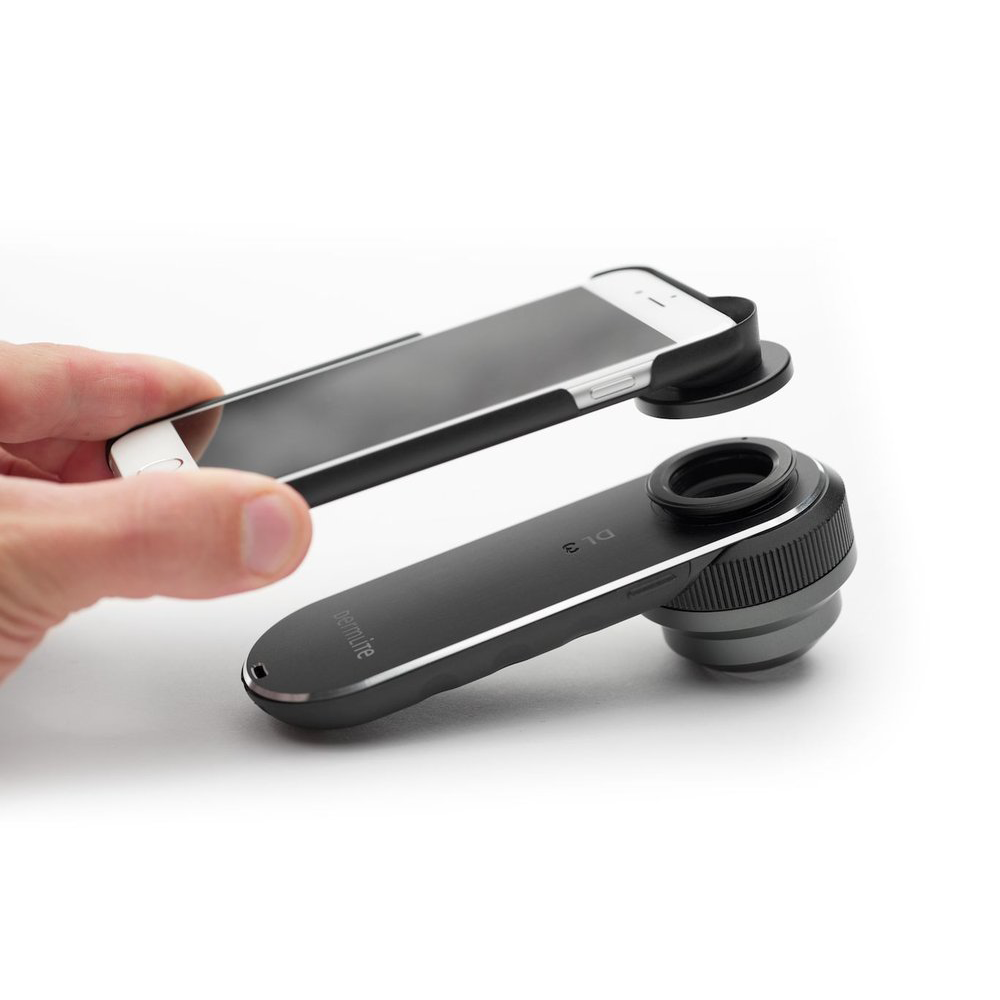
\includegraphics[width=\linewidth]{contents/chapter_2/resources/dermatoscope_example_3.png}
    \end{subfigure}
    \caption{Exemple de dispositifs de dermatoscopie proposé par Dermlite: à gauche le dispositif seul, au milieu ce même dispositif adapté à un appareil photo standard et à droite le dispositif adapté à une caméra de smartphone.}
    \label{fig:dermatoscope_example}
\end{figure}\par

\subsubsection{Microscopie confocale par réflectance}
La \gls{rcm} est une technique d’imagerie décrite durant les années 1950 par Marvin Minsky. Les avancés réalisées durant les années 1990 ont permis de réduire considérablement la taille de cet appareil et de faciliter ainsi son utilisation dans divers domaines. Cette techniques de plus en plus répandue dans les services de dermatologie a également connu un regain de notoriété dans les journaux scientifiques: une recherche à l’aide des mots clés « reflectance confocal microscopy skin » apporte une dizaine de publications en 2000 contre 150 en 2010.\par
\begin{figure}[H]
\centering
    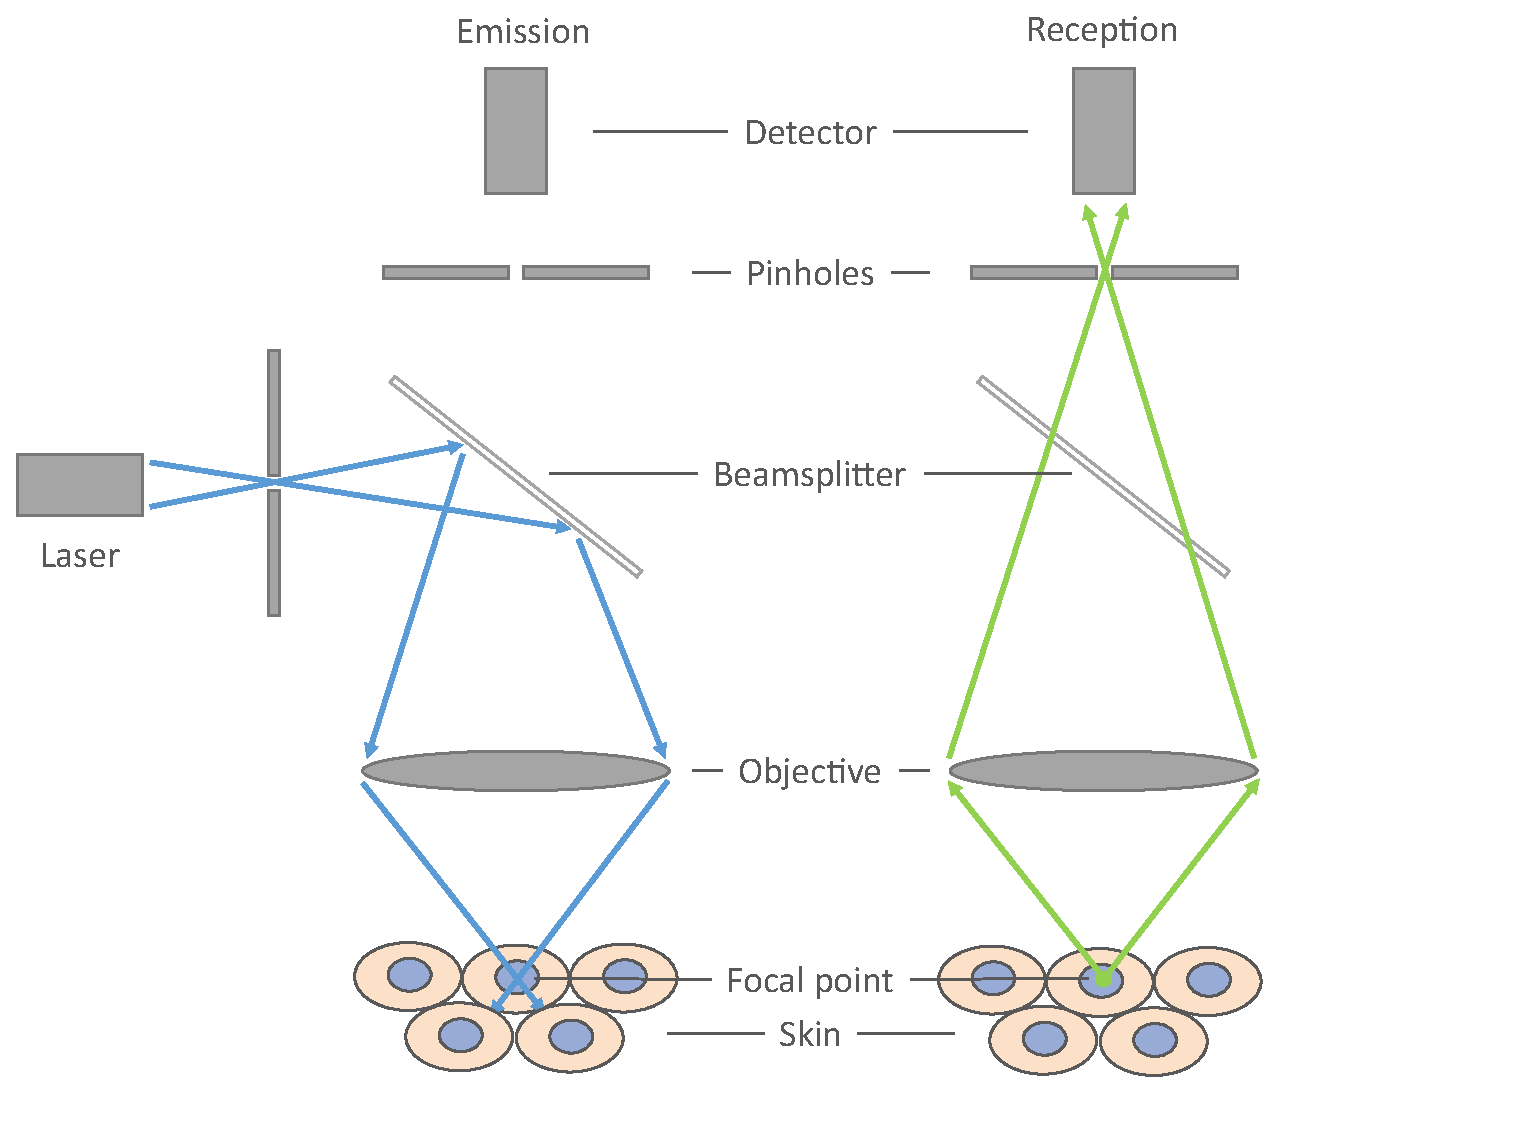
\includegraphics[width=0.6\linewidth]{contents/chapter_2/resources/rcm_principle.pdf}
    \caption{Schéma de fonctionnement du \gls{rcm} en deux temps: un laser est émis et focalisé en un point spécifique de la peau (Émission) puis la lumière est réfléchie et reçue par une caméra au travers d'un trou de faible diamètre (Réception).}
    \label{fig:rcm_principle}
\end{figure}\par
Cette technique emploie l’utilisation d’un sténopé situé devant le capteur et permet de conserver uniquement les photons issus du plan focal choisi, illustré en \Cref{fig:rcm_principle}. Nous pouvons par ce principe, obtenir différents plans focaux ou plans de coupes, participant à l’obtention d’une information 3D. En dermatologie, les dispositifs se basent sur des longueurs d’ondes de \SI{830}{\nano\metre} non invasives pour la peau et les yeux, mais limitent la profondeur de du dispositif à \SIrange{200}{300}{\micro\metre}.\par
Pour finir, à la manière du dermatoscope, un gel à base d’eau de réfraction proche de celle de l’épiderme est utilisé entre la lentille du microscope et la peau afin de limiter la perte de photons et de permettre l’obtention d’image du derme.\par

\subsubsection{Tomographie en cohérence optique}
Initialement conçue pour le domaine de l’ophtalmologie, la \gls{oct} est une technologie récente qui tend à se démocratiser à de nombreux domaines d’intervention dont celui de la dermatologie. Ces dispositifs se basent sur un principe d’interférométrie, préalablement utilisée pour les dispositifs dits d’interférométrie à faible cohérence temporelle fournissant une information à une dimension. Le principe consiste à utiliser une source de lumière commune divisée en deux faisceaux, l’un servant de référence et le second servant à l’analyse de l’échantillon considéré. Le faisceau de référence possède un miroir ajustable, permettant de modifier sa distance parcourue et définissant ainsi la profondeur d’échantillon analysable. En effet, deux faisceaux peuvent interférer si la distance parcourue (et leur déphasage) est identique \Cref{fig:oct_principle}.\par
L’\gls{oct} est une extension de ce principe à deux dimensions, permettant la caractérisation d’une « tranche » de tissu. Cette modalité d’imagerie propose ainsi une information temps réel en profondeur (de l’ordre du millimètre), avec une résolution proche du micromètre. Nous pouvons obtenir, par acquisition de plusieurs plans de coupe, une reconstruction de la peau et de ses structures.\par
\begin{figure}[H]
    \centering
    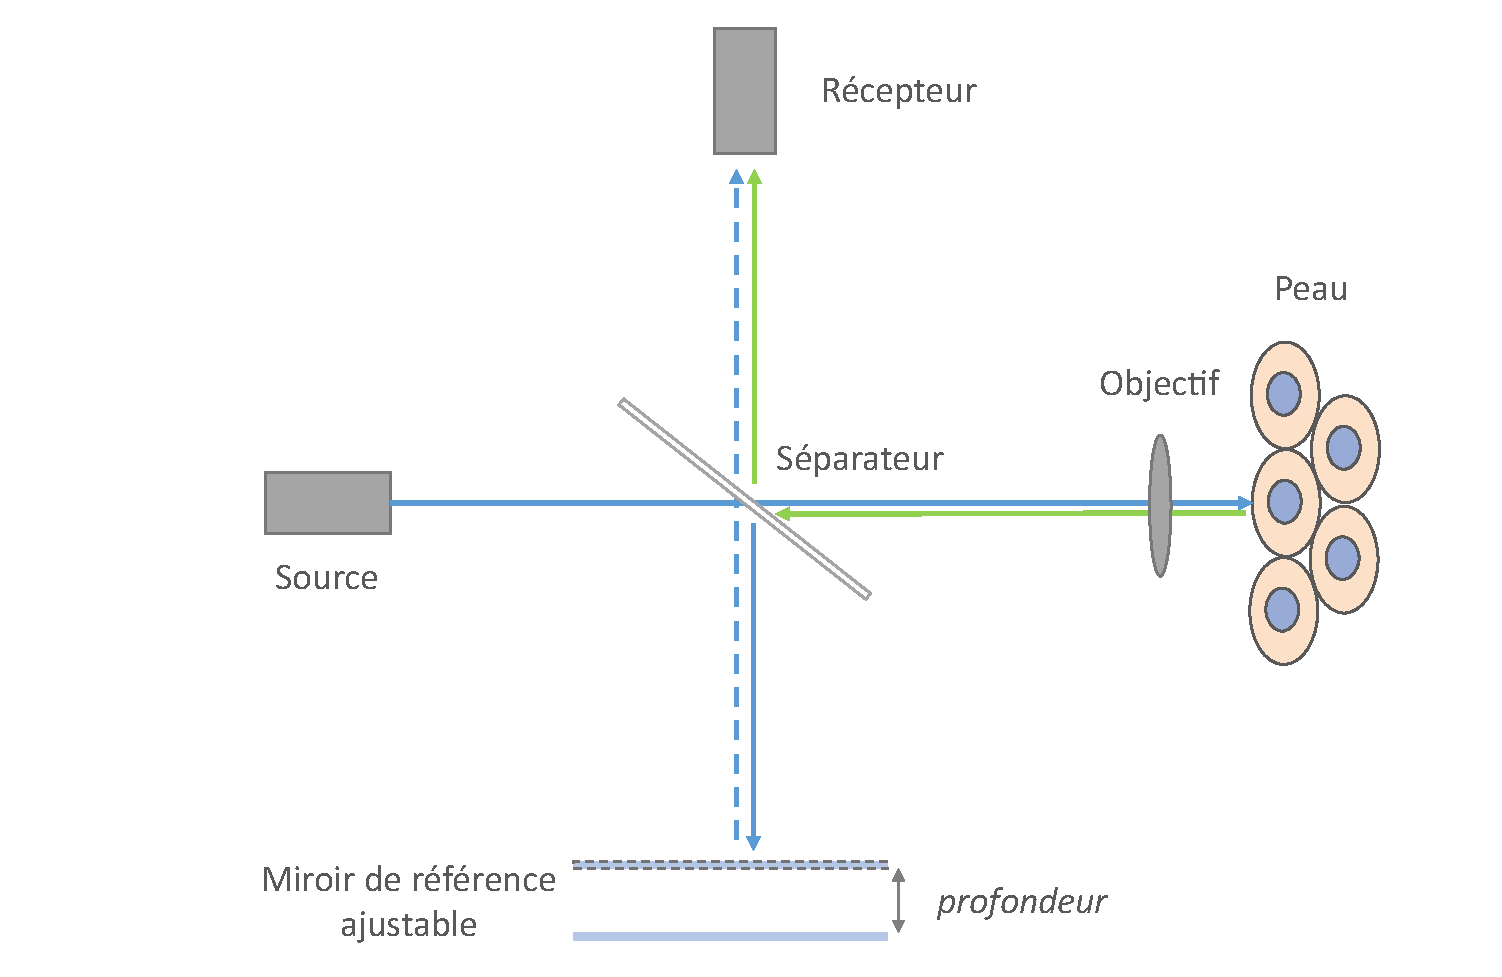
\includegraphics[width=0.8\linewidth]{contents/chapter_2/resources/oct_principle.pdf}
    \caption{Schéma de fonctionnement du \gls{oct}.}
    \label{fig:oct_principle}
\end{figure}\par

\subsubsection{Spectrocopie}
\subsubsection{Microscope confocal Raman}

\subsection{Modalités de mesure non optique}
Nous évoquerons au travers de ces quelques lignes les modalités employées de manière expérimentale. Ces modalités n’interviennent pas dans nos travaux, mais nécessitent d’être évoquées à titre formel.

\subsubsection{Imagerie par résonance magnétique}
\subsubsection{Ultrasons haute fréquence}

\clearpage
\section{Données de travail}
\subsection{Présentation}
Nous traiterons au sein de cette partie de notre "matière" de travail. En effet, l'ensemble de ce travail prend appuie sur une base de données mise à disposition initialement pour la réalisation d'une étude clinique menée sur la pertinence de la dermatoscopie et de la \gls{rcm} en milieu clinique~\cite{Cinotti2018}. Cette base a reçue une autorisation de la part du comité d'éthique du \gls{chu} de Saint-Etienne pour son exploitation au sein de l'étude clinique mentionnée précédemment mais également pour ce travail universitaire (Numéro du comité d'examen institutionnel 672016/CHUSTE).\par 
Cette base de données compile des lésions faciales possédant les critères suivant:
\begin{itemize}
\item les patients ont été acquis entre les années 2011 et 2015 au \gls{chu} de Saint-Etienne
\item les données sont disponibles pour chaque patient sous 3 formes: photographie clinique, dermatoscopie et \gls{rcm}
\item les lésions inclues été supposées de \gls{lm}/\gls{lmm} et le diagnostique différentiel était fortement controversé.
\end{itemize}\par

En terme de composition, la base regroupe 201 patients répartie entre 96 femmes et 105 hommes d'un âge moyen égal à 70 ans compris entre 29 et 97 ans \Cref{fig:statistics}. Cette base comporte 223 lésions uniques dont le diagnostique que nous utiliserons comme référence provient de l'histologie. Ces lésions se décomposent en :
\begin{itemize}
\item 115 malignes : scindée en 92 \gls{lm} et 23 \gls{lmm}
\item 108 bénignes : dont 20 \gls{bcc}, 37 \gls{sl}, 23 \gls{sk}, 15 \gls{pak}, 8 naevus, 2 kératose lichénoïde, 2 cicatrices et 1 maladie de Bowen pigmentée.
\end{itemize}\par

\begin{figure}[H]
    \centering
    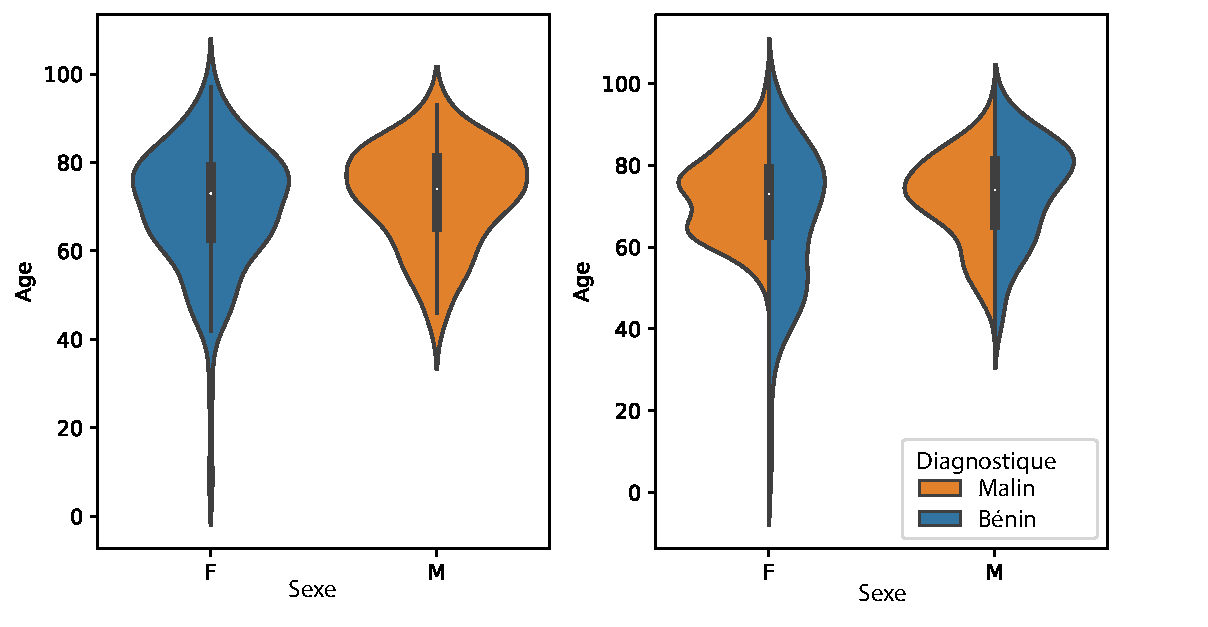
\includegraphics[width=0.8\linewidth]{contents/chapter_2/resources/statistics.pdf}
    \caption{A gauche, répartition en fonction de l'âge et du sexe. A droite, répartition entre l'âge et le sexe en tenant compte du diagnostique binaire.}
    \label{fig:statistics}
\end{figure}\par

En ce qui concerne leur acquisition, celle-ci a à chaque fois été réalisée par l'un des 3 experts investigateurs de l'étude clinique~\cite{Cinotti2018}. Tout cas de collisions de tumeurs au sein d'un même groupe a été exclue de cette étude. En ce qui concerne la modalité de dermatoscopie, les données ont été produites à l'aide d'une caméra PowerShot® G7~\textsuperscript{\ref{footnote:device_powershot}} couplé au dispositif proposé par Fotofinder~\textsuperscript{\ref{footnote:device_fotofinder}}. Pour ce qui est de la modalité de \gls{rcm}, les données proviennent d'une caméra VivaScope 3000®~\textsuperscript{\ref{footnote:device_mavig}}. En revanche, aucune information lié à l'acquisition des données de photographie clinique n'a été mentionnée.\par

\addtocounter{footnote}{1}
\footnotetext[\thefootnote]{Source : Canon Powershot®, Canon, Tokyo, Japon. \label{footnote:device_powershot}}
\addtocounter{footnote}{1}
\footnotetext[\thefootnote]{Source : FotoFinder Systems GmbH, Bad Birnbach, Allemagne. \label{footnote:device_fotofinder}}
\addtocounter{footnote}{1}
\footnotetext[\thefootnote]{Source : Distribué en Europe par MAVIG GmbH, Munich, Allemagne. \label{footnote:device_mavig}}

\subsection{Évaluation des experts}
Afin d'évaluer les performances de praticiens face à ces lésions, les investigateurs ont eu recours à 21 dermatologues détenant une expertise des modalités d'imagerie non invasives. Ces experts sont réparti de manière homogène selon leur compétences respectives pour chacun des dispositifs. Ainsi, le panel d'évaluation se décompose de la façon suivante: 
\begin{inenum}
\item 6 experts sont soumis à l'ensemble des modalités,
\item 15 experts sont soumis à l'évaluation de la photographie clinique et de la dermatoscopie (dont 6 sur l'ensemble et 9 uniques)
\item et 12 sont soumis à la \gls{rcm} (dont 6 sur l'ensemble et 6 uniques)~\cite{Cinotti2018}.
\end{inenum}
Cette situation est résumée en \Cref{fig:experts_evaluation}.
\begin{figure}[H]
    \centering
    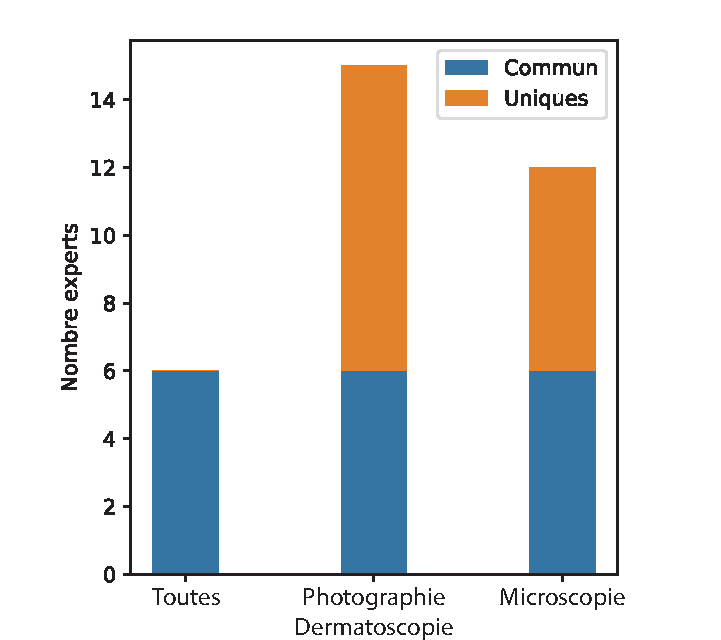
\includegraphics[width=0.4\linewidth]{contents/chapter_2/resources/experts_evaluation.pdf}
    \caption{Répartition du panel de 21 dermatologues sur l'évaluation des diverses modalités~\cite{Cinotti2018}.}
    \label{fig:experts_evaluation}
\end{figure}\par
Pour éviter tout biais dans l'évaluation, les experts évalués sur l'ensemble des modalités ont contactés sur 3 journées différentes: 
\begin{inenum}
\item une première évaluation sur images de photographie clinique et dermatoscopie,
\item une seconde évaluation sur images de \gls{rcm}
\item et une dernière évaluation sur l'ensemble des images.
\end{inenum}
Par ailleurs, les images ont été présentée dans un ordre différents enter chaque journée d'évaluation. De plus, l'évaluation sur base d'image de photographie clinique a toujours été réalisée avant la dermatoscopie.\par

